\documentclass{scrartcl}
\usepackage{graphicx}
\usepackage[utf8]{inputenc}
\usepackage[T1]{fontenc}
\usepackage[frenchb]{babel}
\usepackage{lmodern}
\usepackage{geometry}
\usepackage{enumitem, pifont}
\usepackage{xcolor}
\usepackage{amsfonts}
\usepackage{amssymb}
\usepackage{amsmath}
\usepackage[cache=false]{minted}


\setlist[itemize, 1]{label = {\textbullet},}

\geometry{top=2cm, bottom=2cm, left=2cm, right=2cm}

\begin{document}
    \title{Pavage avec des tatamis}
    \subtitle{Propositon de projet maths-info}
    \author{Bruno Bourgine}
    \maketitle

    \section{Descriptif de la problématique}


    Le pavage du plan avec des rectangle est un problème classique et déjà largement documenté,
    mais je souhaite l'aborder par un aspect très concret : étant donné un nombre de tatamis, quelles sont les 
    configurations possibles.\\
    \begin{center}
        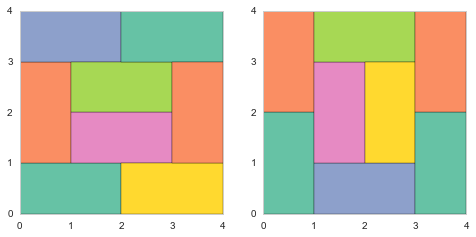
\includegraphics[width = 0.5\linewidth]{pavage-par-tatamis.png}
    \end{center}
    C'est un problème que rencontre notamment toute personne qui se retrouve à devoir installer un dojo.
    Il existe une contrainte de base qui est que 4 tatamis ne rejoignent jamais en un même coin. Mais ont peut
    en ajouter d'autres : possibilité de demi-tatamis (carré), répartition des couleurs, répartition de l'usure...

    \section{Cahier des charges}

    Utilisateur final : gestionnaire de dojo\\

    L'interface utilisateur devra comprendre un menu de paramétrage basique : nombre de tatamis,
    contraintes géométriques, contraintes d'aspect général; ainsi qu'un affichage des dispositions envisageables.\\

    L'utilisateur devra pouvoir saisir :

    \begin{itemize}
        \item le nombre et le type (entier/demis) de tatamis à disposition
        \item leurs dimensions
        \item leurs couleurs
        \item éventuellement leur état (on dispose de préférence les plus usés en périphérie)
        \item les dimensions du dojo
    \end{itemize}

    L'affichage proposera différentes disposition selon les contraintes imposées.


    \section{Langages et outils envisagés}

    La résolution de ce type de problème correspond au champ de la programmation par contraintes. Il s'agira donc 
    dans un premier temps de découvrir (en tout cas en ce qui me concerne) ce paradigme de programmation.\\

    Les langages utilisables sont divers, si ce n'est qu'ils doivent être compatibles
    avec le développement d'une interface graphique sur terminal mobile.
    Le choix se portera plutôt vers python (avec PyQT5 ou Kivy) ou java.\\

    La gestion du projet se déroulera à l'aide de l'outil Redmine, et les fichiers seront gérés à l'aide de la plateforme framagit.


\end{document}
